% Chapter 5

\chapter{Bilan du stage} % 5th chapter title

\label{Chapter5} % For referencing the chapter elsewhere, use \ref{Chapter5} 

%----------------------------------------------------------------------------------------

\section{Ressources utilisées}

Les ressources utilisées durant le stage varient en nature et en fonction.

\subsection{Écriture de code}
\begin{itemize}
 \item \textbf{Visual Studio Code} : Pour l'édition du code en langages C++ et LaTeX grâce à ses nombreuses fonctionnalités. Les extensions CMake, LateX Workshop et LTeX ont considerableme facilite les travaux.
 \item \textbf{Google Colab}: Pour facilitation de l'apprentissage grâce à ses GPU. Les librairies Python les plus utilisées ici sont Numpy, Pandans, et Keras.
 \item \textbf{Jupyter} : Pour les tâches ne nécessitant pas trop de ressource (visualisation, sauvegarde en format PARQUET). Les librairies Python majeures utilisées ici sont Numpy, Pandas et Matplotlib.
 \item \textbf{Kile}: Pour l'écriture du premier brouillon du rapport en Latex.
 \item \textbf{Draw.io} : Pour les illustrations.
\end{itemize}


\subsection{Communication}
Les communications se sont effectuées principalement par messagerie électronique. J'ai aussi eu l'occasion de communiquer avec les professeurs en présentiel à trois reprises.

%----------------------------------------------------------------------------------------

\section{Journal de bord}
\label{sec:Journal}

\subsection{Semaines 1 et 2}
\begin{itemize}
 \item 15 juin: Réunion de début de Stage par Google Meet.
 \item 16 juin: Demande aux professeurs de vérifier un exemple de simulation 1D, avant de me lancer la génération des données.
 \item 17 juin: Remarque du problème de formation et de propagation d'un créneau indésirable sur l'énergie, le flux et la température.
 \item 18 juin: Rédaction d'un nouveau schéma par M. Franck (pour l'étape 1) qui devrait conserver l'équilibre.
 \item 22 juin: Détection de la source du problème d'apparition du créneau indésirable, et définition d'un nouveau terme $S^\prime$. 
 \item 23 juin: Confirmation de l'exactitude des simulations 1D et début de la génération des données avec 500 mailles.
 \item 25 juin: Demande d'aide à M. Vigon pour la configuration de la fonction d'activation de la couche de sortie sous Keras.
\end{itemize}


\subsection{Semaines 3 et 4}

\begin{itemize}
 \item 3 juillet: Rencontre avec M. Navoret pour discuter des avancements. Prise de connaissance d'une des raisons potentielles du problème de mauvaise prédiction de la position du créneau sur la densité en 1D. Proposition de plusieurs solutions par M. Navoret, entre autre de partir d'un signal stationnaire sinusoïdal et d'introduire l'onde à un temps t*>0.
 \item 6 juillet: Nouvelles simulations effectuées en vue d'observer la différence entre les effets de deux densités différentes. Continuation vers des nouvelles simulations avec 300 mailles.
 \item 8 juillet: Décroissance du taux d'apprentissage à la suggestion de M. Franck mais non-amélioration des résultats d'apprentissage.
 \item 9 juillet: Passage aux réseaux convolutif grâce à M. Vigon.
 \item 11 juillet: Plot du début des oscillations, des maximum, des minimum à la demande de M. Vigon, afin de mieux observer les effets de deux créneaux de densités différentes. 
\end{itemize}

\subsection{Semaines 5 et 6}

\begin{itemize}
 \item 13 juillet: Rencontre avec M. Navoret et M. Franck à la fac. Devant la persistance du problème de non-détection de la position du créneau, l'implémentation du problème en 2D semble être la solution appropriée.
 \item 14 juillet Reformulation 2D du schéma de « splitting » et adaptation du code 1D en 2D.
 \item 19 juillet: Fin du codage 2D et présentation des résultats.
 \item 25 juillet: Ajustement de la gamme de couleurs pour les visualisations et passage à la génération des données sur 90x90 mailles.
\end{itemize}

\subsection{Semaines 7, 8, et 9}
\begin{itemize}
 \item 5 août: Rencontre avec M. Franck à la fac. Proposition de solutions pour la non-détection de la position du créneau en 2D par résolution d'un système proche de l'équation de la chaleur, après affichage par lignes de niveaux. La possibilité d'adopter un obstacle s'étendant sur toute la verticale est envisagée. Prise de connaissance des délais pour la rédaction du rapport.
 \item 6 août: Rédaction et envoi du plan du rapport de stage. 
 \item 7 août: Proposition de réduction drastique de la résolution spatiale, et proposition de nouvelles idées par M. Vigon, entre autre la considération d'un obstacle considérable plus opaque.
 \item 8 août: Nouvel apprentissage avec des simplifications majeures qui fonctionne. Amélioration des résultats et continuation du rapport.
 \item 15 août: Soumission du premier brouillon du rapport.
\end{itemize}
%----------------------------------------------------------------------------------------

\section{Difficultés rencontrées et solutions apportées}

Un résume du déroulement du stage est présente à la figure \ref{fig:MilestonesRoadmap}. Les points les plus marquants du stage y sont représentés. On peut aussi y voire les difficultés majeures auxquelles j'ai été confronte.

\begin{figure}[H] 
\centering
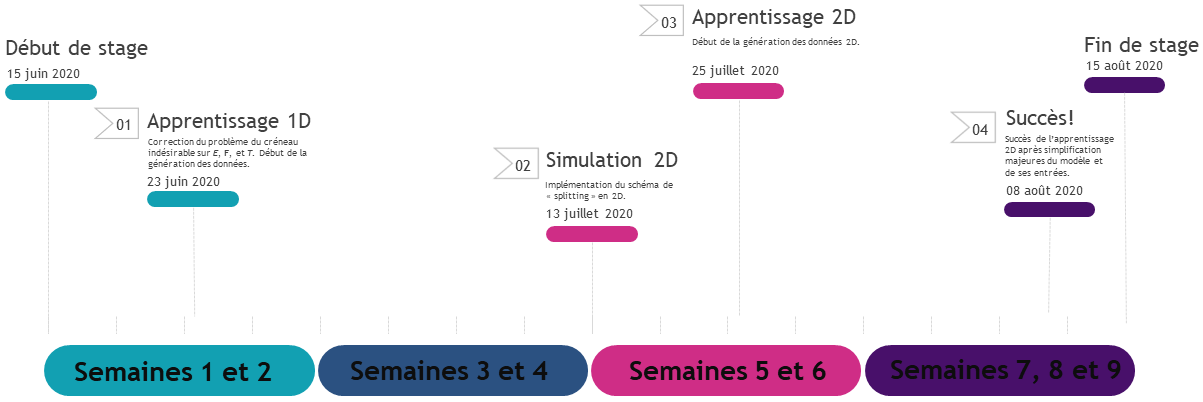
\includegraphics[width=.8\linewidth]{MilestonesRoadmap} 
\decoRule
\caption[MilestonesRoadmap]{Résumés des tournants du stage. Les détails du déroulement peuvent être obtenues dans la section \ref{sec:Journal}.}
\label{fig:MilestonesRoadmap}
\end{figure}

\subsection{Apparition d'un créneau indésirable}
Au commencement du stage, le code de calcul 1D n'était pas au point. En effet, dès qu'on plaçait un créneau sur la densité, un créneau correspondant se formait puis se propageait sur les signaux $E$, $F$, et $T$. Le problème a été résolu par rajout d'un terme $S^\prime$ au niveau de la deuxième équation du schéma de « splitting ».

\subsection{Detection de la position du crenau}
La détection de la position du saut de densité a été un problème récurant durant le stage. À la fin stage, aucune solution (si elle existe) n'a été trouvée pour le problème inverse en 1D. Cependant en 2D le problème a été résolu par diminution du taux d'apprentissage à $1e-5$ et augmentation du nombre d'époques. Il est bien connu que l'entrainement des réseaux de neurones peu diverger si le taux d'apprentissage est trop élevé. Quant au nombre d'époques, je n'en faisais pas suffisamment pour voir le modèle converger. Une solution bien plus rapide aurait été d'automatiser la recherche des hyper-paramètres, chose que je n'ai apprise qu'à la fin du stage.

Pour revenir à l'apprentissage en 1D, il est important de mentionner de façon spéculative quelques pistes d'étude qui, bien combinée, peuvent améliorer les résultats 1D:
\begin{itemize}
    \item \textbf{deux apprentissages différents} : en créant un modèle sépare pour l'apprentissage de la position et un autre pour la hauteur
    \item \textbf{élimination des mauvais labels} : on pourrait supprimer de l'apprentissage tous les exemples qui ont un label trop proche du bord du domaine (par exemple ne garder que ceux compris entre 0.2 et 0.8 comme en 2D).
\end{itemize}

Cela dit, la solution trouvée en 2D est loin d'être optimale ; elle souffre de deux problèmes majeurs :
\begin{itemize}
 \item \textbf{pas de generalisation} : le modèle finalement retenu ne comporte pas de couche de max-pooling qui aurait probablement aidé a la généralisation. Aucun test n'a été fait pour vérifier le niveau de généralisation de ce modèle.
 \item \textbf{model trop lourd} : le nombre de paramètres est très élevé dû à la taille des entrées \verb|(168, 28, 48)|, ce qui necessite un espace memoire tres important au moment de la sauvegarde des poids (2Go).
\end{itemize}

Toutes ces quatre pistes d'amélioration n'ont pas été implémentées pour cause de temps. En effet, la gestion de temps a été un vrai problème tout au long du stage.

\subsection{Gestion du temps}
La gestion du temps durant le stage n'a pas été facile. Au moment d'implémenter le schéma en 2D (ce qui n'était pas initialement prévu), j'ai longuement hésiter sur l'option la plus rapide. J'ai pu compter sur les conseils de M. Navoret pour surmonter cet obstacle. 

Aussi, je me suis rendu compte des délais bien en retard, j'ai du me débrouiller pour terminer l'apprentissage et améliorer les résultats tout en rédigeant le rapport. Cela dit, je n'ai pas réussi à faire une partie essentielle qui consiste à étudier l'apport du max-pooling dans la généralisation du modèle de CNN.

%----------------------------------------------------------------------------------------

\section{Les apports du stage}

Ce stage a été enrichissant pour moi sur plusieurs fronts :

\subsection{Expérience en développement}
J'ai gagné de l'expérience en développement C++ et Python, tout en me développant un portfolio. J'ai beaucoup appris sur l'API de Pandas, Matplotlib, et de Keras. J'ai à présent une large base de données de code réutilisable pour d'autres taches.

\subsection{Équations aux dérivées partielles}
J'ai pu observer directement quelques astuces utilisées par MM. Navoret et Franck pour vérifier la validité d'une simulation. Pour l'équation du transfert radiatif, j'ai compris la nécessité de partir d'un état d'équilibre radiatif.

\subsection{Réseaux de neurones}
Ce stage m'a permis de percevoir la puissance des réseaux de neurones. J'ai appris à quel point le taux d'apprentissage est important, comme le rappelle cette citation du livre de référence Deep Learning : \textit{"The learning rate is perhaps the most important hyperparameter. If you have time to tune only one hyperparameter, tune the learning rate."} \parencite[417]{Reference5}. 

Tous ces enseignements me poussent à me poser quelques questions concernant le « batch size ». Lors de l'apprentissage, il a fallu entrainer le modèle en utilisant la méthode d' \textbf{augmentation du « batch size »} pour obtenir les premiers "bons" résultats. Cette méthode référencée \href{https://arxiv.org/pdf/1711.00489.pdf}{ici} montre que beaucoup de questions restent à résoudre dans le domaine du Deep Learning.

\subsection{Expérience de recherche}
En tant que première expérience dans un environnement de recherche tel que l'UFR, j'ai pu me familiariser avec le milieu. J'ai notamment appris que les résultats ne doivent pas toujours être ceux auxquels on s'attend, du moment que l'on a une explication pour l'échec.

%----------------------------------------------------------------------------------------
